\documentclass[../Syllabus.tex]{subfiles}

\begin{document}

\section{Chapitre 2 : Class Diagram}

\subsection{Motivation}

Un Class Diagram exprime les caractéristiques statiques des différents éléments d'un Système d'Information. Il tire son origine du paradigme de programmation Orienté Objet. Les spécifications du programme final dérivent du modèle ainsi construit.

Lors de la conception du modèle, le système sera décomposé en une multitude de petits composants. Cette approche permet un gain considérable au niveau de la complexité, mais aussi au niveau des utilisations futures. En effet, les différents concepts générés pourront être réutilisés pendant tout le développement et même durant d'autres projets. D'autre part, le modèle est plus facilement modifiable qu'un code source. On peut progressivement modifier le modelling pour le faire correspondre aux attentes.

\subsection{Modélisation Orienté Objet}

L'idée principale de la Modélisation Orienté Objet est de décrire le Système d'Information sur base des objets le constituant. Les différentes méthodes d'interaction entre ces objets sont ajoutées au modèles.

Un objet représente un élément possédant :

\begin{itemize}
  \item Une \textbf{identité} : l'élément existe dans le système modélisé.
  \item Une \textbf{durée de vie} : l'élément existe pour une période donnée.
  \item Un \textbf{état} : l'élément possède des caractéristiques à un moment donné.
  \item Une \textbf{pertinence} et une \textbf{signification} : tous deux établis dans le domaine et décris dans le glossaire.
\end{itemize}

\begin{figure}[htp]
    \centering
    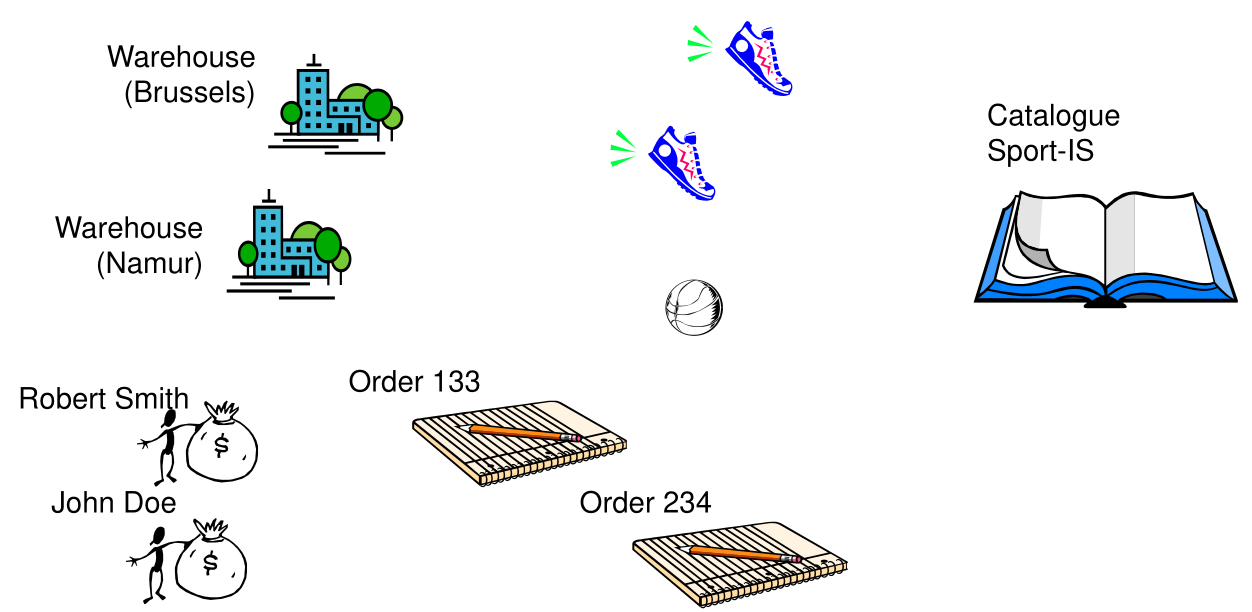
\includegraphics[width=13cm]{./img/chapter2-step1.png}
    \caption{Les différents éléments du SI.}
    \label{fig:chapter2-step1}
\end{figure}

\begin{figure}[htp]
    \centering
    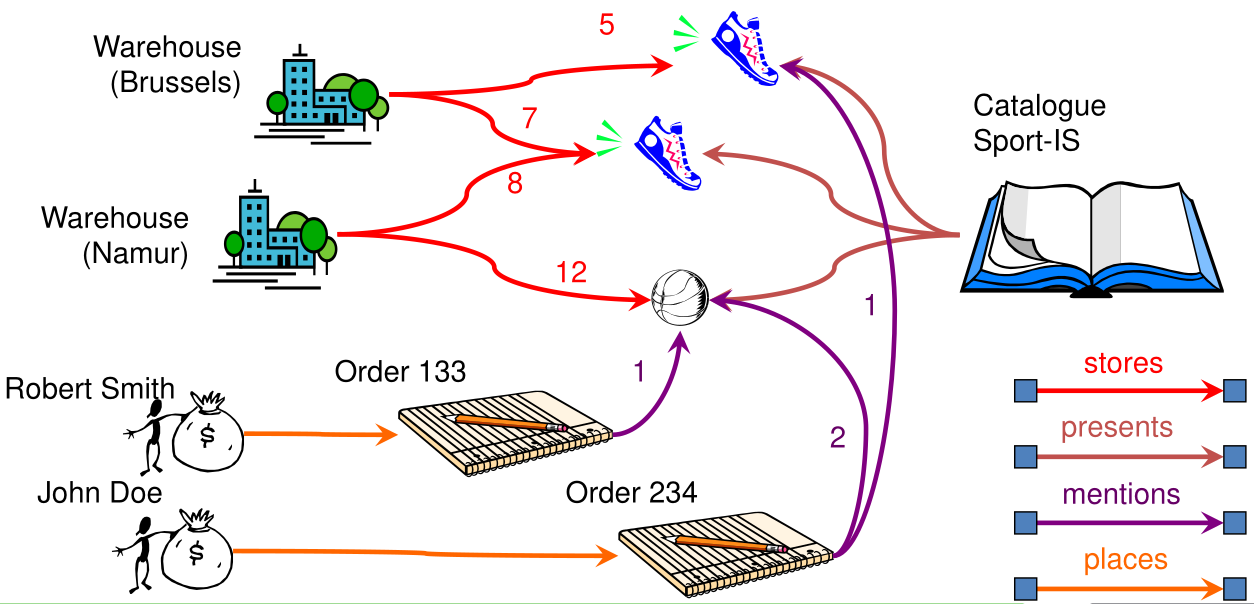
\includegraphics[width=13cm]{./img/chapter2-step2.png}
    \caption{Les interactions entre les différents objets sont représentées.}
    \label{fig:chapter2-step2}
\end{figure}

\subsection{Classification}

Le Système d'Information peut être composé de millions de différents éléments qui ne peuvent pas être représentés de manière individuelle dans le modèle. Les Class permettent de décomposer ce monde en un ensemble d'objets partageant des caractéristiques communes et pertinentes.

Une notion de granularité est présentée. Les classes représentes donc des ensembles d'éléments avec des caractéristiques communes. Pourtant des différences sont présentes entre ces différents éléments. Le modèle peut choisir des les ignorer ou de les prendre en compte à plus ou moins haut niveau. Cette granularité est définie pour regarder le monde d'une manière différente. Un exemple pour cette granularité : pour un supermarché, modéliser un système d'information prenant en compte la couleur des sodas n'est pas pertinent au niveau de la gestion des stocks (mais pourrait être pertinent dans une gestion marketing).

\begin{figure}[htp]
    \centering
    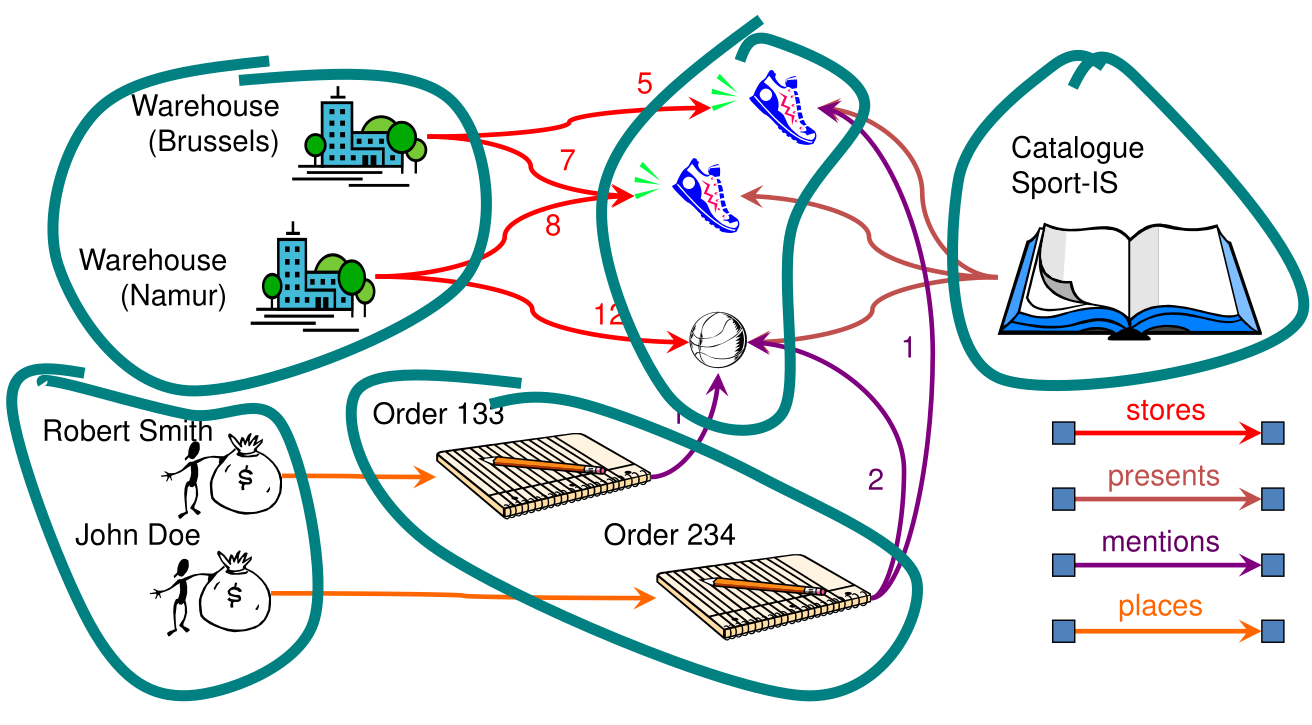
\includegraphics[width=13cm]{./img/chapter2-step3.png}
    \caption{Les objets sont classés selon la granularité choisie.}
    \label{fig:chapter2-step3}
\end{figure}

\begin{figure}[htp]
    \centering
    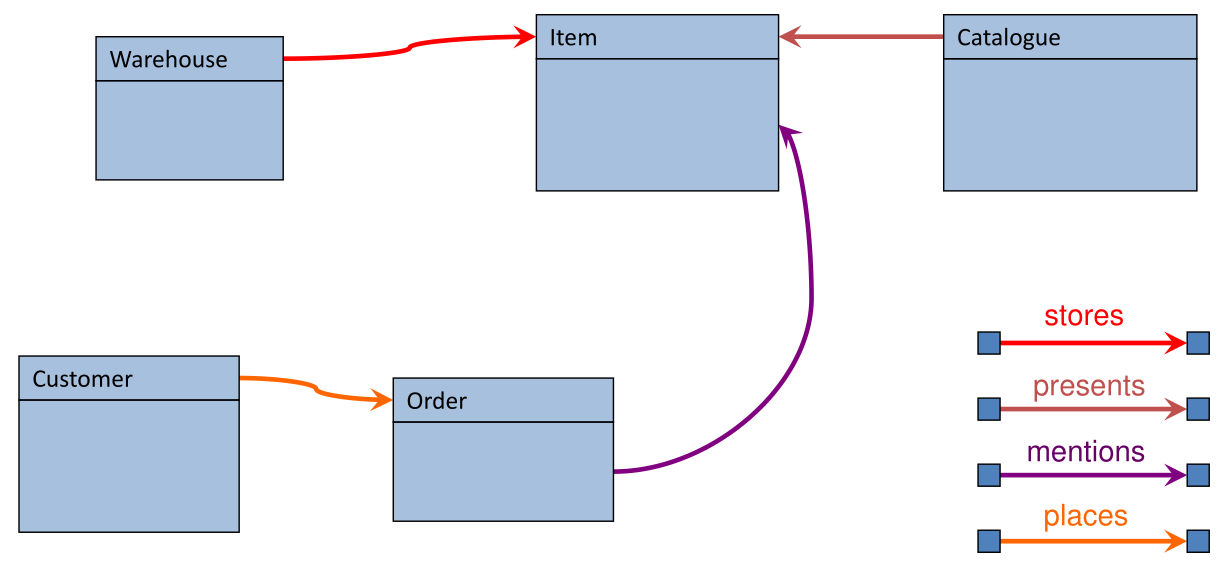
\includegraphics[width=13cm]{./img/chapter2-step4.png}
    \caption{Les différentes classes extraites du SI.}
    \label{fig:chapter2-step4}
\end{figure}

\clearpage

\subsection{Programmation et Syntaxe}

Une Class (au sens programmation du terme) agit comme une structure de donnée possédant des caractéristiques et des méthodes agissant sur ces données. \textit{In object-oriented programming, a class is an extensible program-code-template for creating objects, providing initial values for state (member variables) and implementations of behavior (member functions or methods)}. Une instance est un objet construit sur base de cette classe et partage donc l'ensemble de ses caractéristiques et méthodes. Exemple :

\begin{figure}[htp]
    \centering
    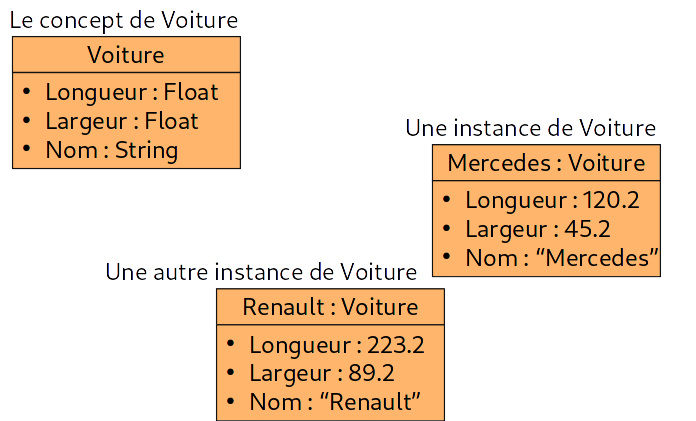
\includegraphics[width=10cm]{./img/chapter2-class-instance.png}
    \caption{Exemple de relation entre class et instance de class.}
    \label{fig:chapter2-class-instance}
\end{figure}

Le cours original utilise la notation UML pour les diagrames de classes. On y retrouve les concepts fondamentaux de la programmation orienté objet. Ces concepts ne seront pas explicités dans ce syllabus et sont jugés assimilés par notre cher lecteur. Si toutefois un doute persiste, contactez les auteurs et priez bien fort le Dieu de la JVM.

Les différents attributs de la classe :

\fbox{[+/-/\texttildelow/\#] \textit{NomDeLAttribut} : \textit{Type} (= \textit{ValeurInitiale})}

La valeur initiale est facultative.

\begin{itemize}
  \item \textbf{+} : Visibilité \textit{public}
  \item \textbf{-} : Visibilité \textit{private}
  \item \textbf{\texttildelow} : Visibilité \textit{package}
  \item \textbf{\#} : Visibilité \textit{protected}
\end{itemize}

Les différentes méthodes de la classe (reprenant les mêmes règles de visibilité reprise précédemment) :

\fbox{[+/-/\texttildelow/\#] \textit{NomDeLaMéthode}(\textit{NomDArgument} : \textit{TypeDArgument}) (: \textit{Type})}

Le type de la méthode est facultatif si la fonction ne renvoie rien. Les arguments aussi si ceux-ci sont absents.

\begin{figure}[htp]
    \centering
    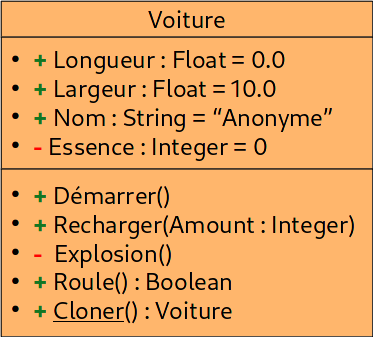
\includegraphics[width=5cm]{./img/chapter2-uml-example.png}
    \caption{Exemple d'une classe décrite dans une notation UML.}
    \label{fig:chapter2-uml-example}
\end{figure}

Un attribut ou une méthode peut être déclaré \textit{static}, c'est-à-dire que sa valeur est identique pour toutes les instances de cette classe. Pour rendre un élément \textit{static}, il suffit de le souligner.

% TODO PAGE160 On doit vraiment parler de ça ?

\subsection{Relations}

Expliciter les relations entre les différents objets du Système d'Information permet de relier et de structurer les concepts entre eux et d'organiser une hierarchie.

\subsubsection{Association}

Une association explicite le lien entre deux classes. Une association est caractérisée par :

\begin{itemize}
  \item \textbf{Nom} : Nom de l'association.
  \item \textbf{Rôle} : Rôle de chacune des deux classes de l'associations. Le rôle possède aussi une visibilité ([+/-/\texttildelow/\#]).
  \item \textbf{Direction de lecture} : Direction de l'association (relative au nom).
  \item \textbf{Multiplicité} : Nombre d'instance pouvent être associées entre elles (0,1,[0..n], [n..n], etc).
\end{itemize}

Dans l'exemple qui suit, nous pouvons lire une association de la manière suivante : \textit{Une facture référence une ou plusieurs pièces de voiture et cette pièce de voiture est une entrée dans zéro ou une facture}, \textit{Un client paie une ou plusieurs facture et une facture est payée par un seul client}, \textit{etc}.

\begin{figure}[htp]
    \centering
    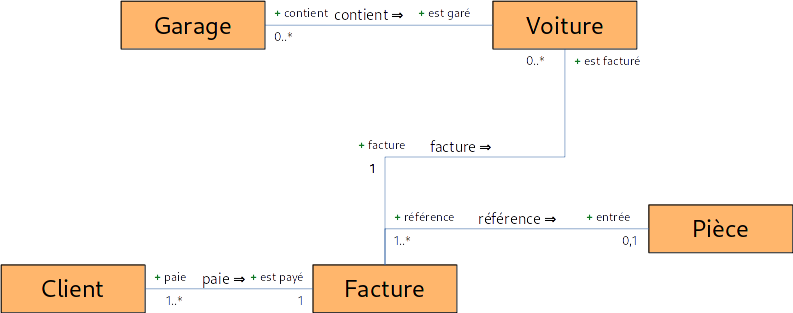
\includegraphics[width=16cm]{./img/chapter2-associations.png}
    \caption{Exemple d'associations.}
    \label{fig:chapter2-associations}
\end{figure}

% TODO: ajouter les relations n-aires ?

\subsubsection{Aggrégation et Composition}

Un type particulier d'association utilisé quand une instance de classe peut être perçu comme un aggrégat/groupe d'autres instances. La relation est donc formée par un Aggrégat et par un Composant.

\begin{figure}[htp]
    \centering
    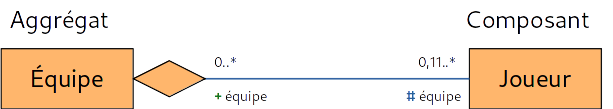
\includegraphics[width=12cm]{./img/chapter2-aggregat.png}
    \caption{Exemple d'un aggrégat.}
    \label{fig:chapter2-aggregat}
\end{figure}

La composition est une forme plus simple de l'aggrégation où le Composant ne peut exister sans l'Aggrégat. Quelques contraintes sont présentes. Un aggrégat ne peut avoir qu'une multiplicité de 1 et un composant ne peut être en relation que dans une seule composition.

\begin{figure}[htp]
    \centering
    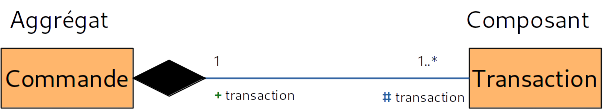
\includegraphics[width=12cm]{./img/chapter2-composition.png}
    \caption{Exemple d'une composition.}
    \label{fig:chapter2-composition}
\end{figure}

% TODO: doit-on parler des N-aray again ?

\subsubsection{Généralisation et Spécialisation}

La généralisation et la spécialisation permettent de construire une hierarchie dans les relations. Cette hierarchie se traduira par un genre d'héritage entre les différentes classes. La relation est construite par une Superclass jugée \textit{générale} et une Subclass jugée \textit{spécialisée}.

\begin{figure}[htp]
    \centering
    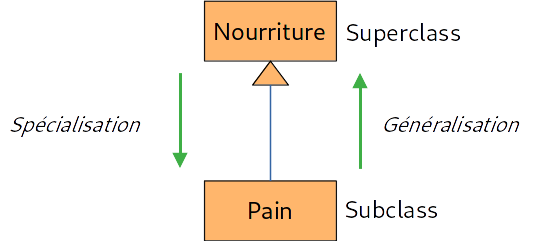
\includegraphics[width=12cm]{./img/chapter2-generalisation.png}
    \caption{Exemple d'une généralisation.}
    \label{fig:chapter2-generalisation}
\end{figure}

L'intérêt de la spécialisation est d'ajouter des caractéristiques inhérantes à la Subclass et donc de se focaliser sur des détails qui ne sont pas pertinents pour la Superclass. Bien sûr, la généralisation permet l'effet inverse : une factorisation par l'extraction des caractéristiques communes pour permettre une conception plus générique.

\begin{figure}[htp]
    \centering
    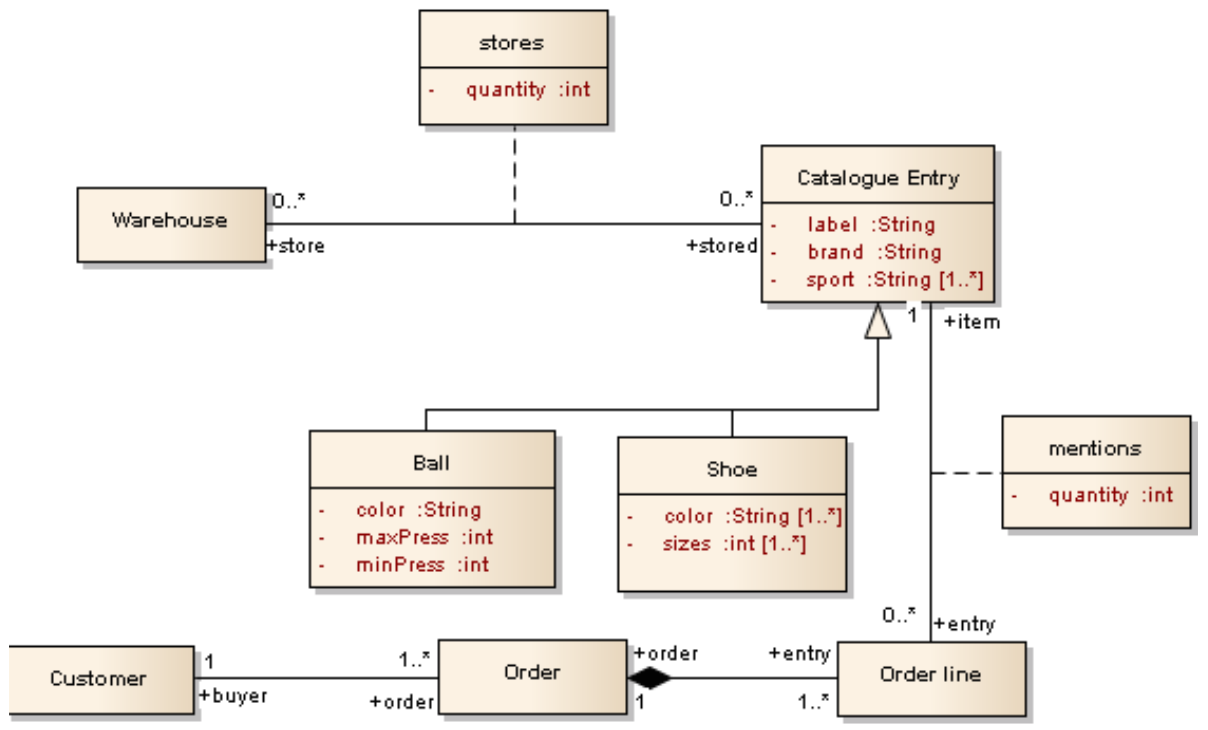
\includegraphics[width=14cm]{./img/chapter2-generalisation2.png}
    \caption{Inclusion d'une généralisation dans un modèle de SI.}
    \label{fig:chapter2-generalisation}
\end{figure}

Les généralisations et spécialisations peuvent être caractérisées sur deux dimensions :

\begin{itemize}
  \item \textbf{Complete} : Chaque instance de la Superclass est aussi une instance d'une Subclass.
  \item \textbf{Incomplete} : Toutes les instances d'une Superclass ne sont pas forcément une instance d'une Subclass.
\end{itemize}

\begin{figure}[htp]
    \centering
    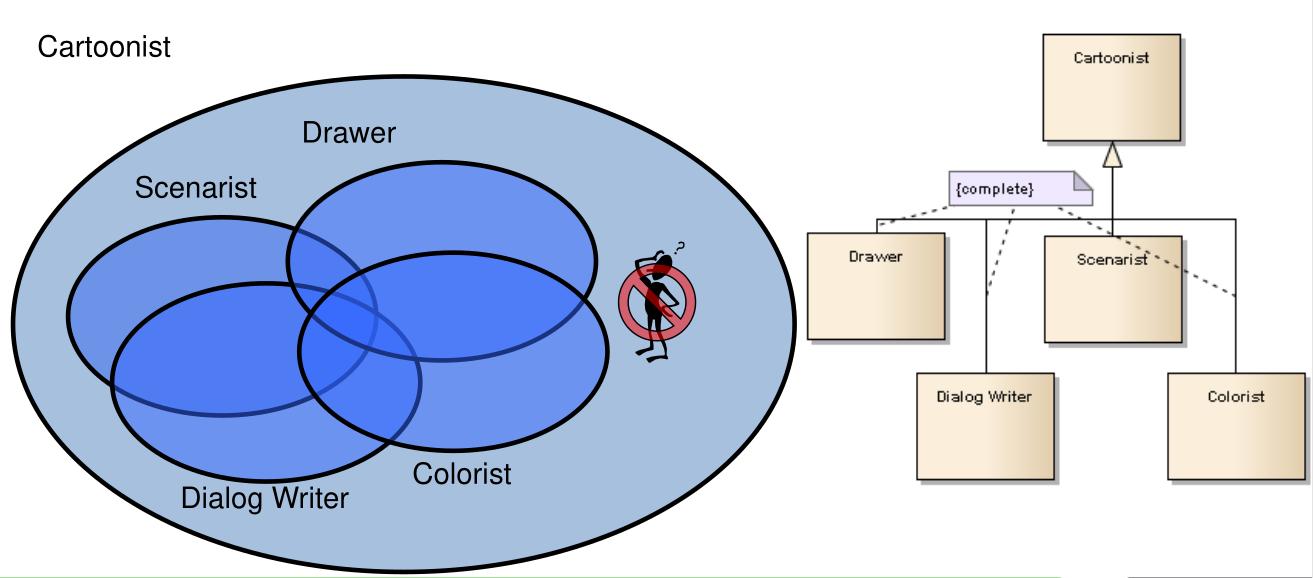
\includegraphics[width=14cm]{./img/chapter2-complete.png}
    \caption{Exemple de complete.}
    \label{fig:chapter2-complete}
\end{figure}

\begin{figure}[htp]
    \centering
    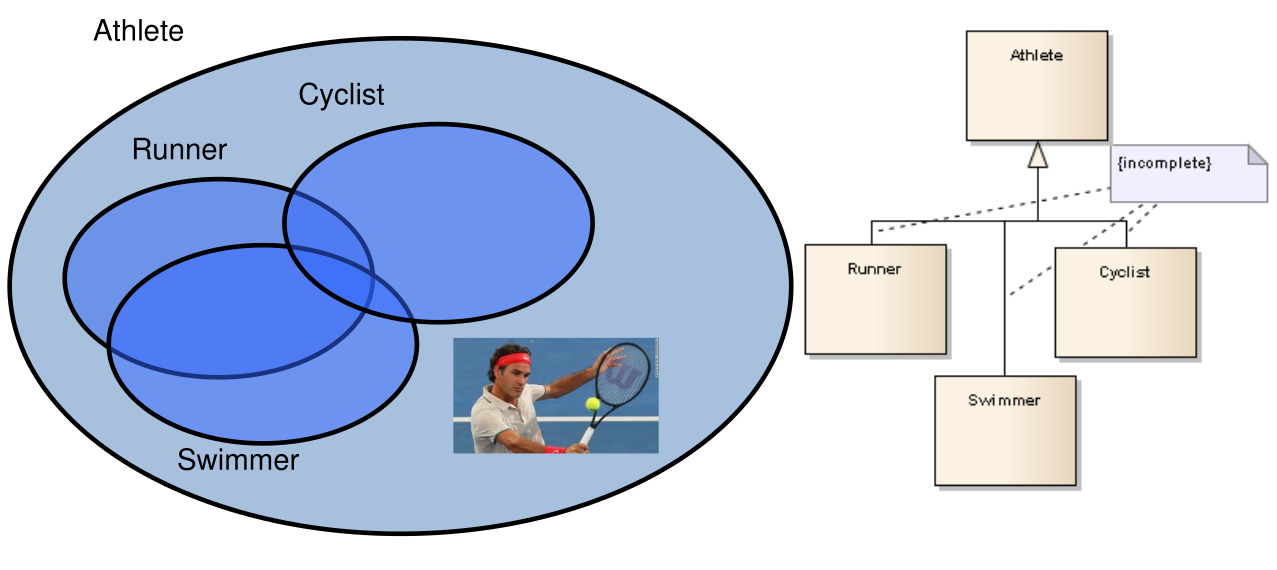
\includegraphics[width=14cm]{./img/chapter2-incomplete.png}
    \caption{Exemple d'incomplete.}
    \label{fig:chapter2-incomplete}
\end{figure}

\begin{itemize}
  \item \textbf{Overlapping} : Il y a au moins une instance de la Superclass qui est aussi une instance de deux Subclasses ou plus.
  \item \textbf{Disjoint} : Il n'y a aucune instance de la Superclass qui est une instance de plus d'une Subclass.
\end{itemize}

\begin{figure}[htp]
    \centering
    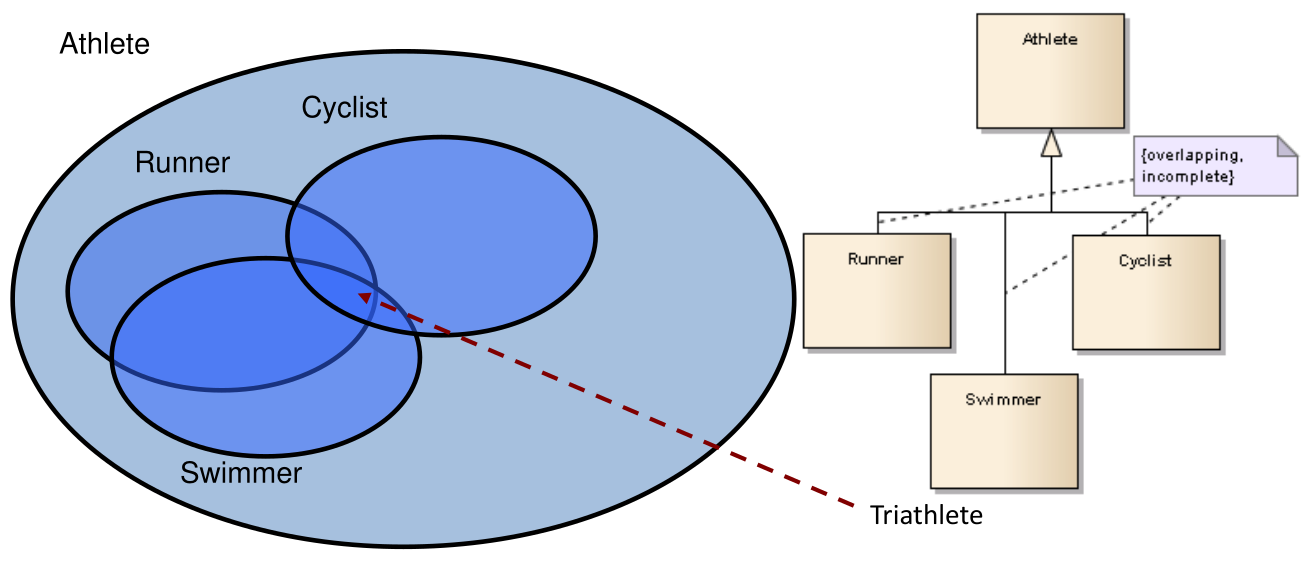
\includegraphics[width=14cm]{./img/chapter2-overlapping.png}
    \caption{Exemple d'overlapping.}
    \label{fig:chapter2-overlapping}
\end{figure}

\begin{figure}[htp]
    \centering
    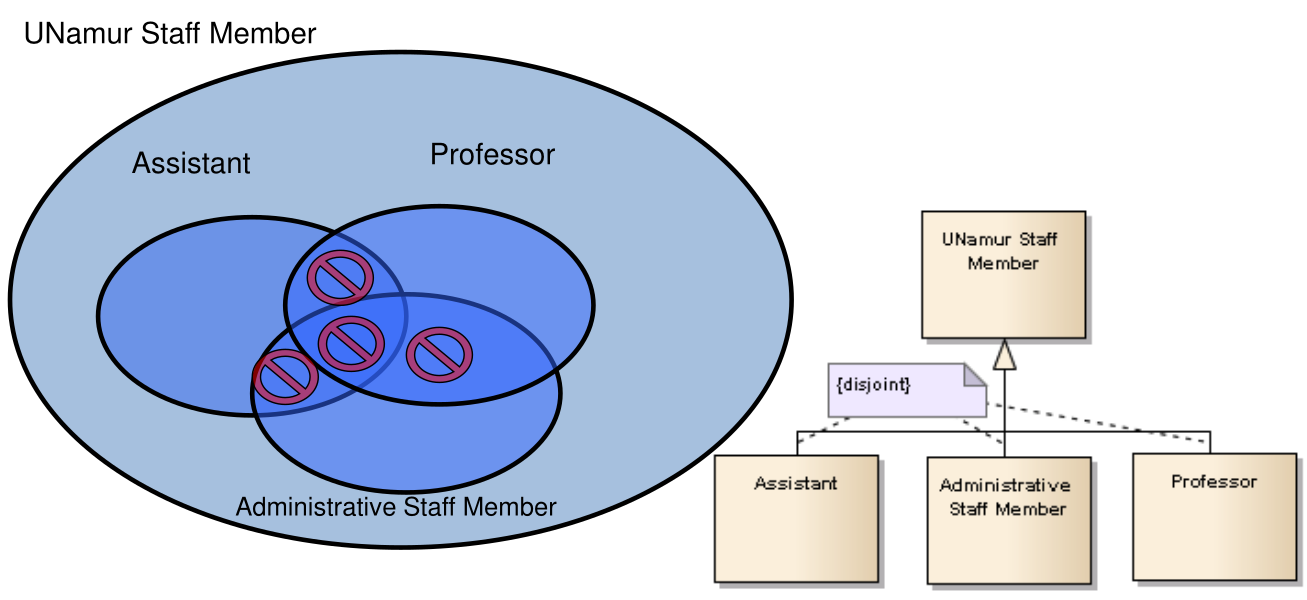
\includegraphics[width=14cm]{./img/chapter2-disjoint.png}
    \caption{Exemple de disjoint.}
    \label{fig:chapter2-generalisation}
\end{figure}

\clearpage

\subsubsection{Dépendances}

Wow manque d'info crucial.

\subsection{Classe abstraite}

Lorsqu'une Superclass ne peut être instanciée qu'à travers ses Subclass, celle-ci est déclarée \textit{abstract} (et \textit{concrete} si c'est n'est pas le cas). Les classes abstraites sont aussi accompagnées de méthode et les méthodes elles-même peuvent être abstraites. Une méthode abstraite est une méthode non implémentée et les Subclasses de cette Superclass doivent donc l'implémenter. Il suffit pour une class de déclarer une seule méthode abstraite pour que la classe elle-même soit jugée abstraite.

Une classe ne devrait pas fournir une implémentation pour une opération si cette opération est abstraite ou si l'implémentation fournie par la Superclass est pertinente.

\subsection{Interface}

Une interface est une ensemble d'attributs et de méthodes publiques qu'une class peut fournir à/exiger d'autres classes. UML fournit une syntaxe pour exprimer cet héritage de méthodes quelque peu spécial.

\begin{figure}[htp]
    \centering
    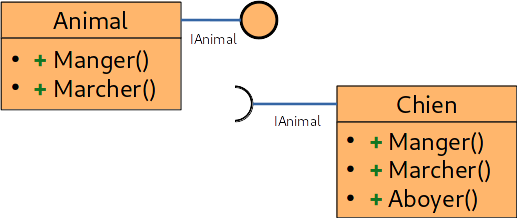
\includegraphics[width=14cm]{./img/chapter2-interface.png}
    \caption{Exemple d'interface.}
    \label{fig:chapter2-interface}
\end{figure}

\end{document}
